\section{Conclusion}

Norway is actually 100\% aligned with the European NIS Directive. However, there is little evidence that Norway has identified its \acrshort{oes} according to EU's guideline.

\begin{followup}
  Outline the complexities navigaating the different documents and legislations in the EU and Norway.

  There are many stakeholders, authorities and agencies, that regulates and sets policies. Often with over lapping responsibilities and objectives. Making passing policies and implmenting policies complicated.
  
  Many Member states must adhere to and align both National and EU NIS Directive when establishing or revising their NCSS. Again, adding to complexity and GAPS.

  A mix and differing definitions and terminologies are bing used and are not always aligned with each other. Making translation of policies tricker. There is a lack of formal and standardised definitons on most cases.
\end{followup}


% \includesvg{tex/Studio_1_Activity_Diagram.svg}
% 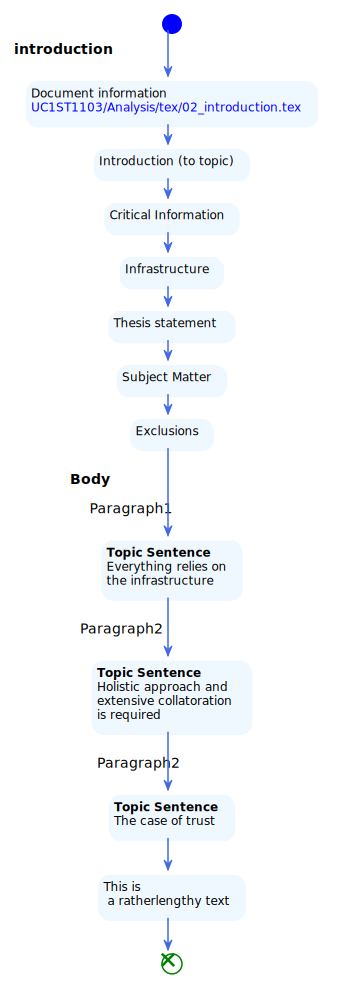
\includegraphics{tex/Studio_1_Activity_Diagram.png}


